\documentclass[11pt,a4paper]{article}

\usepackage[utf8]{inputenc}
\usepackage[T1]{fontenc}
\usepackage{mathpazo}
\usepackage[scaled=0.92]{helvet}
\usepackage[margin=1in]{geometry}
\usepackage{graphicx}
\usepackage{amsmath,amssymb,amsfonts}
\usepackage{booktabs}
\usepackage{tabularx}
\usepackage{setspace}
\usepackage{titlesec}
\usepackage{fancyhdr}
\usepackage{float}
\usepackage{caption}
\usepackage{microtype}

\usepackage{tikz}
\usetikzlibrary{shapes.geometric, arrows.meta, positioning, calc, matrix, fit, backgrounds}

\usepackage{listings}
\usepackage{xcolor}
\usepackage[hidelinks]{hyperref}

\setstretch{1.15}
\setlength{\parindent}{0pt}
\setlength{\parskip}{0.8em}
\sloppy

\titleformat{\section}{\normalfont\large\bfseries\sffamily}{\thesection}{1em}{}
\titleformat{\subsection}{\normalfont\normalsize\bfseries\sffamily}{\thesubsection}{1em}{}
\titleformat{\subsubsection}{\normalfont\normalsize\itshape\sffamily}{\thesubsubsection}{1em}{}

\pagestyle{fancy}
\fancyhf{}
\fancyhead[L]{\small\sffamily Fondasi Basis Data: Tipe Data SQL dan Tipe Primitif}
\fancyhead[R]{\small\sffamily\thepage}
\renewcommand{\headrulewidth}{0.4pt}

\captionsetup{font=small,labelfont=bf,labelsep=period}

\renewenvironment{abstract}
{\small
	\begin{center}\textbf{\sffamily Abstrak}\end{center}
	\begin{quote}}
	{\end{quote}}

\lstdefinestyle{code}{
	basicstyle=\ttfamily\small,
	frame=single,
	rulecolor=\color{black},
	breaklines=true,
	showstringspaces=false,
	columns=fullflexible,
	keepspaces=true,
	framesep=6pt,
	aboveskip=1em,
	belowskip=1em,
	xleftmargin=0pt
}

\lstdefinestyle{out}{
	basicstyle=\ttfamily\small,
	frame=tb,
	rulecolor=\color{black},
	breaklines=true,
	showstringspaces=false,
	columns=fullflexible,
	keepspaces=true,
	framesep=4pt,
	aboveskip=1em,
	belowskip=1em
}

\title{\vspace{-1.5cm}\textbf{\sffamily\LARGE Fondasi Basis Data: Tipe Data SQL dalam Perspektif Tipe Primitif Rust dan Zig}}
\author{
	\textbf{Muhammad Riduwan Khafidi} \\
	\small Program Studi Teknik Rekayasa Perangkat Lunak \\
	\small Politeknik Negeri Batam \\
	\small \texttt{4342611034@students.polibatam.ac.id}
}
\date{\small\today}

\begin{document}

\maketitle
\thispagestyle{empty}

\begin{abstract}
	Tipe data SQL sering diajarkan sebagai daftar hafalan yang terpisah dari dunia pemrograman sistem. Padahal, bagi seorang pengembang yang akrab dengan tipe primitif seperti \texttt{u8}, \texttt{i32}, \texttt{f32}, atau \texttt{f64} di Rust dan Zig, tipe data SQL dapat dipahami sebagai \textit{padanan tingkat penyimpanan} dari tipe-tipe tersebut. Makalah ini menyajikan pemetaan sistematis dan visual antara tipe primitif Rust dan Zig dengan tipe data SQL, mulai dari integer bertanda dan tak bertanda, bilangan pecahan IEEE-754, boolean, string, hingga data biner tetap. Setiap konsep dilengkapi ilustrasi bit-level, langkah per langkah, dan contoh output nyata agar pembaca yang belum pernah menyentuh database dapat memahami \textit{mengapa} setiap tipe ada, bukan hanya \textit{apa} namanya. Pembaca akan memperoleh kerangka mental yang utuh untuk memilih tipe data secara sadar.
\end{abstract}

\section{Pendahuluan: Mengapa Harus Peduli pada Tipe Data?}

\subsection{Cerita Pembuka: Warung Nasi dan Buku Kas}

Bayangkan kamu punya warung nasi. Setiap hari kamu mencatat pesanan pelanggan. Ada dua pilihan:

\begin{itemize}
	\item \textit{Cara A:} mencatat semuanya di satu buku tulis besar, tanpa kolom, tanpa format. Cepat menulis, tetapi saat ingin menghitung total pendapatan hari ini, kamu harus membaca ulang semuanya secara manual.
	\item \textit{Cara B:} mencatat di buku kas dengan kolom rapi: Tanggal, Nama Menu, Jumlah, Harga, Total. Lebih lambat saat menulis, tetapi saat butuh laporan, kamu bisa langsung menghitung.
\end{itemize}

Basis data memaksa kita memilih Cara B. Kolom Jumlah hanya boleh diisi angka, bukan teks "dua piring". Kolom Tanggal hanya boleh diisi tanggal, bukan "kemarin sore". Aturan inilah yang disebut tipe data.

\subsection{Tipe Data sebagai Kontrak}

Ketika kamu menulis:

\begin{lstlisting}[style=code]
CREATE TABLE pesanan (
    jumlah INT,
    harga  DECIMAL(10,2)
);
\end{lstlisting}

kamu sedang membuat kontrak dengan database: kolom \texttt{jumlah} hanya akan menerima bilangan bulat, dan jika ada yang mencoba memasukkan teks, database akan menolak. Kontrak ini punya tiga manfaat nyata:

\begin{enumerate}
	\item Mencegah data sampah. Tidak ada yang bisa memasukkan \texttt{'dua piring'} ke kolom \texttt{jumlah}.
	\item Menghemat ruang. Angka \texttt{25} disimpan sebagai 4 byte, sedangkan teks \texttt{'dua puluh lima'} butuh 15 byte.
	\item Mempercepat perhitungan. Database bisa langsung menjumlahkan \texttt{jumlah * harga} tanpa perlu mengubah teks menjadi angka.
\end{enumerate}

\subsection{Jembatan ke Rust dan Zig}

Di Rust, kamu menulis:

\begin{lstlisting}[style=code]
let usia: u8 = 25;
let saldo: i64 = -150000;
let rasio: f64 = 0.75;
\end{lstlisting}

Tiga baris itu membuat tiga kontrak yang persis sama dengan SQL: \texttt{u8} berarti bilangan bulat 0--255, \texttt{i64} berarti bilangan bulat 64-bit bertanda, \texttt{f64} berarti bilangan pecahan 64-bit. Yang berbeda hanyalah tempat kontrak itu ditulis. Di Rust, kontrak diperiksa saat kompilasi. Di SQL, kontrak disimpan di katalog database dan diperiksa saat \texttt{INSERT}.

Tesis makalah ini: tipe data SQL adalah tipe primitif yang disimpan secara permanen. Memahami satu sisi mempermudah memahami sisi lainnya.

\section{Peta Keluarga Tipe Data SQL}

Secara garis besar, tipe data SQL terbagi menjadi lima keluarga. Gambar~\ref{fig:tree} memetakan keluarga tersebut secara visual.

\begin{figure}[H]
	\centering
	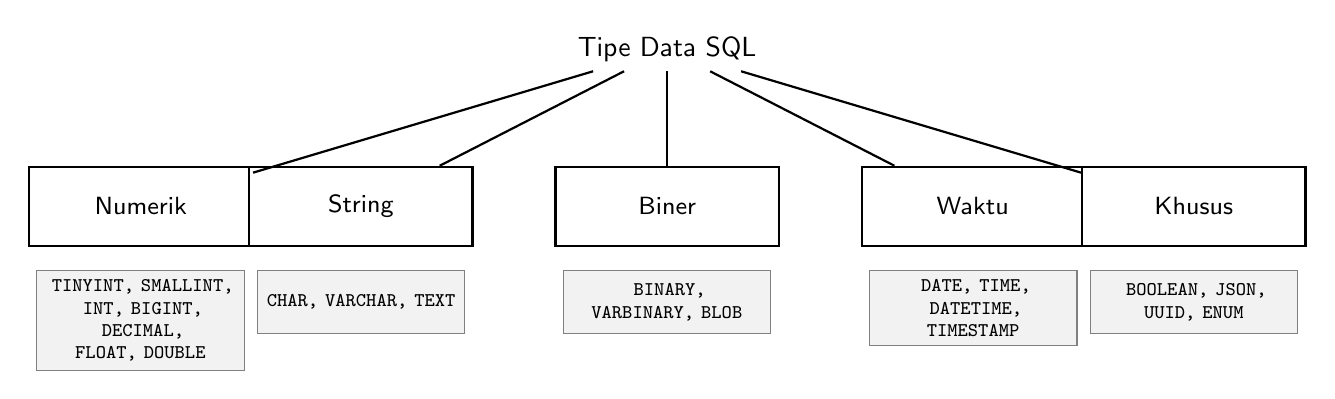
\begin{tikzpicture}[
			node distance=0.5cm and 0.8cm,
			cat/.style={rectangle, draw=black, thick, fill=white, text width=2.6cm, align=center, minimum height=1cm, font=\sffamily\small},
			leaf/.style={rectangle, draw=black!50, fill=black!5, text width=2.4cm, align=center, minimum height=0.8cm, font=\ttfamily\scriptsize},
			line/.style={draw, thick}
		]
		\node[font=\sffamily] (root) {Tipe Data SQL};
		\node[cat, below left=1.2cm and 4cm of root] (num) {Numerik};
		\node[cat, below left=1.2cm and 1.2cm of root] (str) {String};
		\node[cat, below=1.2cm of root] (bin) {Biner};
		\node[cat, below right=1.2cm and 1.2cm of root] (time) {Waktu};
		\node[cat, below right=1.2cm and 4cm of root] (misc) {Khusus};

		\draw[line] (root) -- (num);
		\draw[line] (root) -- (str);
		\draw[line] (root) -- (bin);
		\draw[line] (root) -- (time);
		\draw[line] (root) -- (misc);

		\node[leaf, below=0.3cm of num] (l1) {TINYINT, SMALLINT, INT, BIGINT, DECIMAL, FLOAT, DOUBLE};
		\node[leaf, below=0.3cm of str] (l2) {CHAR, VARCHAR, TEXT};
		\node[leaf, below=0.3cm of bin] (l3) {BINARY, VARBINARY, BLOB};
		\node[leaf, below=0.3cm of time] (l4) {DATE, TIME, DATETIME, TIMESTAMP};
		\node[leaf, below=0.3cm of misc] (l5) {BOOLEAN, JSON, UUID, ENUM};
	\end{tikzpicture}
	\caption{Peta keluarga tipe data SQL.}
	\label{fig:tree}
\end{figure}

\section{Integer: Bilangan Bulat dengan Ukuran Bertingkat}

\subsection{Analogi Kotak Berukuran Berbeda}

Bayangkan kamu punya lima jenis kotak: kotak mungil (1 byte), kotak kecil (2 byte), kotak sedang (3 byte), kotak besar (4 byte), dan kotak raksasa (8 byte). Kalau kamu hanya perlu menyimpan satu baju, memakai kotak raksasa berarti membuang ruang sembilan belas baju. Sebaliknya, memakai kotak mungil untuk menyimpan sepuluh baju akan membuat baju tidak muat.

Inilah alasan SQL menyediakan banyak ukuran integer: agar kita bisa memilih kotak yang pas.

\subsection{Representasi Bit-Level}

Sebelum masuk ke tabel, mari lihat bagaimana komputer menyimpan angka. Satu byte terdiri dari 8 bit, setiap bit bernilai 0 atau 1.

\begin{figure}[H]
	\centering
	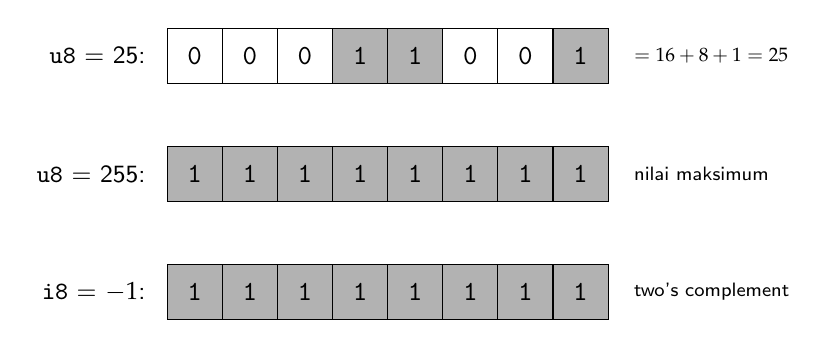
\begin{tikzpicture}[
			bit/.style={rectangle, draw=black, minimum width=0.7cm, minimum height=0.7cm, font=\ttfamily},
			lbl/.style={font=\sffamily\small}
		]
		\node[lbl, anchor=east] at (-0.5, 1.5) {\texttt{u8} = 25:};
		\node[bit, fill=white]    (b7) at (0,1.5) {0};
		\node[bit, fill=white]    (b6) at (0.7,1.5) {0};
		\node[bit, fill=white]    (b5) at (1.4,1.5) {0};
		\node[bit, fill=black!30] (b4) at (2.1,1.5) {1};
		\node[bit, fill=black!30] (b3) at (2.8,1.5) {1};
		\node[bit, fill=white]    (b2) at (3.5,1.5) {0};
		\node[bit, fill=white]    (b1) at (4.2,1.5) {0};
		\node[bit, fill=black!30] (b0) at (4.9,1.5) {1};
		\node[font=\scriptsize\sffamily, right=0.2cm of b0] {$= 16+8+1 = 25$};

		\node[lbl, anchor=east] at (-0.5, 0) {\texttt{u8} = 255:};
		\node[bit, fill=black!30] (c7) at (0,0) {1};
		\node[bit, fill=black!30] (c6) at (0.7,0) {1};
		\node[bit, fill=black!30] (c5) at (1.4,0) {1};
		\node[bit, fill=black!30] (c4) at (2.1,0) {1};
		\node[bit, fill=black!30] (c3) at (2.8,0) {1};
		\node[bit, fill=black!30] (c2) at (3.5,0) {1};
		\node[bit, fill=black!30] (c1) at (4.2,0) {1};
		\node[bit, fill=black!30] (c0) at (4.9,0) {1};
		\node[font=\scriptsize\sffamily, right=0.2cm of c0] {nilai maksimum};

		\node[lbl, anchor=east] at (-0.5, -1.5) {\texttt{i8} = $-1$:};
		\node[bit, fill=black!30] (d7) at (0,-1.5) {1};
		\node[bit, fill=black!30] (d6) at (0.7,-1.5) {1};
		\node[bit, fill=black!30] (d5) at (1.4,-1.5) {1};
		\node[bit, fill=black!30] (d4) at (2.1,-1.5) {1};
		\node[bit, fill=black!30] (d3) at (2.8,-1.5) {1};
		\node[bit, fill=black!30] (d2) at (3.5,-1.5) {1};
		\node[bit, fill=black!30] (d1) at (4.2,-1.5) {1};
		\node[bit, fill=black!30] (d0) at (4.9,-1.5) {1};
		\node[font=\scriptsize\sffamily, right=0.2cm of d0] {two's complement};
	\end{tikzpicture}
	\caption{Representasi bit-level untuk \texttt{u8} dan \texttt{i8}.}
	\label{fig:bit-int}
\end{figure}

Perhatikan Gambar~\ref{fig:bit-int}: \texttt{u8} bernilai 25 disimpan sebagai \texttt{00011001}. Kalau bobotnya dijumlahkan, $16 + 8 + 1 = 25$. Nilai maksimum \texttt{u8} adalah 255 karena semua bit terisi satu. Sementara \texttt{i8} menyimpan $-1$ sebagai \texttt{11111111} karena memakai representasi \textit{two's complement}, di mana bit paling kiri (paling signifikan) menandakan negatif.

Alasan \texttt{u8} berhenti di 255 dan \texttt{i8} berhenti di 127 adalah karena pada \texttt{i8} satu bit "dibuang" untuk menyimpan tanda. Rentang negatifnya adalah $-128$ hingga $-1$, dan positifnya $0$ hingga $127$.

\subsection{Tabel Lengkap Ukuran Integer}

\begin{table}[H]
	\centering
	\caption{Rentang nilai tipe integer di MariaDB dan MySQL.}
	\label{tab:int-sql}
	\small
	\begin{tabular}{l r r r}
		\toprule
		Tipe SQL           & Ukuran & Signed                                       & Unsigned                        \\
		\midrule
		\texttt{TINYINT}   & 1 byte & $-128$ s/d $127$                             & $0$ s/d $255$                   \\
		\texttt{SMALLINT}  & 2 byte & $-32.768$ s/d $32.767$                       & $0$ s/d $65.535$                \\
		\texttt{MEDIUMINT} & 3 byte & $-8.388.608$ s/d $8.388.607$                 & $0$ s/d $16.777.215$            \\
		\texttt{INT}       & 4 byte & $-2{,}1 \times 10^9$ s/d $2{,}1 \times 10^9$ & $0$ s/d $4{,}2 \times 10^9$     \\
		\texttt{BIGINT}    & 8 byte & $\pm 9{,}2 \times 10^{18}$                   & $0$ s/d $1{,}84 \times 10^{19}$ \\
		\bottomrule
	\end{tabular}
\end{table}

\subsection{Pemetaan ke Rust dan Zig}

\begin{table}[H]
	\centering
	\caption{Pemetaan tipe integer Rust dan Zig ke tipe SQL.}
	\label{tab:int-map}
	\small
	\begin{tabular}{l l l l}
		\toprule
		Rust / Zig    & Padanan SQL                & Rentang                      & Kapan Dipakai                    \\
		\midrule
		\texttt{u8}   & \texttt{TINYINT UNSIGNED}  & $0$--$255$                   & Status 0/1, bendera              \\
		\texttt{i8}   & \texttt{TINYINT}           & $-128$--$127$                & Suhu, selisih kecil              \\
		\texttt{u16}  & \texttt{SMALLINT UNSIGNED} & $0$--$65.535$                & Kode pos, tahun                  \\
		\texttt{i16}  & \texttt{SMALLINT}          & $\pm 32.767$                 & ---                              \\
		\texttt{u32}  & \texttt{INT UNSIGNED}      & $0$--$4{,}2 \times 10^9$     & ID umum                          \\
		\texttt{i32}  & \texttt{INT}               & $\pm 2{,}1 \times 10^9$      & ID, jumlah transaksi             \\
		\texttt{u64}  & \texttt{BIGINT UNSIGNED}   & $0$--$1{,}84 \times 10^{19}$ & ID besar, \texttt{UUID\_SHORT()} \\
		\texttt{i64}  & \texttt{BIGINT}            & $\pm 9{,}2 \times 10^{18}$   & Saldo, epoch milidetik           \\
		\texttt{u128} & \texttt{DECIMAL(39,0)}     & $0$--$3{,}4 \times 10^{38}$  & Tidak native                     \\
		\bottomrule
	\end{tabular}
\end{table}

\subsection{Dampak Ukuran Integer pada Performa}

Ini pertanyaan yang sering terlewat: mengapa tidak memakai \texttt{BIGINT} untuk semua hal saja, toh 8 byte tidak seberapa?

Jawabannya: setiap indeks sekunder menyalin primary key. Gambar~\ref{fig:index-dup} mengilustrasikannya.

\begin{figure}[H]
	\centering
	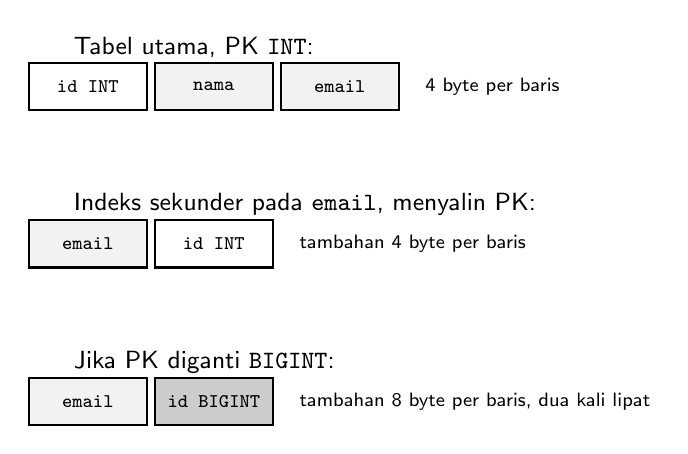
\begin{tikzpicture}[
			tbl/.style={rectangle, draw=black, thick, minimum width=1.5cm, minimum height=0.6cm, font=\ttfamily\scriptsize},
			lbl/.style={font=\sffamily\small},
			note/.style={font=\scriptsize\sffamily}
		]
		\node[lbl, anchor=west] at (-0.3, 2.5) {Tabel utama, PK \texttt{INT}:};
		\node[tbl, fill=white]     (t1) at (0,2)   {id INT};
		\node[tbl, fill=black!5]   (t2) at (1.6,2) {nama};
		\node[tbl, fill=black!5]   (t3) at (3.2,2) {email};
		\node[note, right=0.2cm of t3] {4 byte per baris};

		\node[lbl, anchor=west] at (-0.3, 0.5) {Indeks sekunder pada \texttt{email}, menyalin PK:};
		\node[tbl, fill=black!5]   (i1) at (0,0)   {email};
		\node[tbl, fill=white]     (i2) at (1.6,0) {id INT};
		\node[note, right=0.2cm of i2] {tambahan 4 byte per baris};

		\node[lbl, anchor=west] at (-0.3, -1.5) {Jika PK diganti \texttt{BIGINT}:};
		\node[tbl, fill=black!5]   (j1) at (0,-2)   {email};
		\node[tbl, fill=black!20]  (j2) at (1.6,-2) {id BIGINT};
		\node[note, right=0.2cm of j2] {tambahan 8 byte per baris, dua kali lipat};
	\end{tikzpicture}
	\caption{Ukuran primary key diduplikasi pada setiap indeks sekunder.}
	\label{fig:index-dup}
\end{figure}

Pada tabel sepuluh juta baris dengan tiga indeks sekunder, PK \texttt{INT} membutuhkan tambahan sekitar 120 MB, sedangkan PK \texttt{BIGINT} membutuhkan sekitar 240 MB. Selisih 120 MB di disk. Aturan praktisnya: pilih tipe integer terkecil yang masih menampung seluruh kemungkinan nilai selama umur sistem.

\section{Bilangan Pecahan: \texttt{FLOAT}, \texttt{DOUBLE}, dan \texttt{DECIMAL}}

\subsection{Mengapa \texttt{0.1 + 0.2} Tidak Selalu Sama dengan \texttt{0.3}}

Ini adalah kejutan pertama yang dialami hampir semua programmer. Bilangan desimal seperti \texttt{0.1} sebenarnya tidak bisa direpresentasikan secara persis dalam biner. Sama seperti $1/3 = 0.3333\ldots$ tidak bisa ditulis lengkap dalam desimal, \texttt{0.1} dalam biner adalah \texttt{0.0001100110011\ldots} yang berulang tanpa henti.

Ketika disimpan sebagai \texttt{f32} dengan 23 bit mantissa, angka itu dipotong di bit ke-23. Ketika dijumlahkan dengan \texttt{0.2} yang juga dipotong, hasilnya bukan \texttt{0.3} persis, melainkan \texttt{0.30000001\ldots}

\begin{figure}[H]
	\centering
	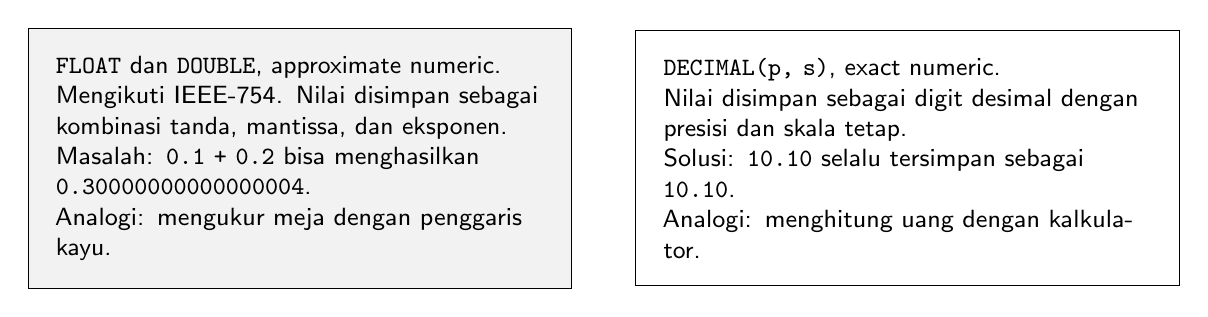
\begin{tikzpicture}[
			box/.style={rectangle, draw=black, text width=6.2cm, align=left, font=\sffamily\small, inner sep=10pt}
		]
		\node[box, fill=black!5] (float) {
			\texttt{FLOAT} dan \texttt{DOUBLE}, approximate numeric. \\
			Mengikuti IEEE-754. Nilai disimpan sebagai kombinasi tanda, mantissa, dan eksponen. \\
			Masalah: \texttt{0.1 + 0.2} bisa menghasilkan \texttt{0.30000000000000004}. \\
			Analogi: mengukur meja dengan penggaris kayu.
		};
		\node[box, fill=white, right=0.8cm of float] (dec) {
			\texttt{DECIMAL(p, s)}, exact numeric. \\
			Nilai disimpan sebagai digit desimal dengan presisi dan skala tetap. \\
			Solusi: \texttt{10.10} selalu tersimpan sebagai \texttt{10.10}. \\
			Analogi: menghitung uang dengan kalkulator.
		};
	\end{tikzpicture}
	\caption{Perbandingan filosofis \texttt{FLOAT}/\texttt{DOUBLE} dengan \texttt{DECIMAL}.}
	\label{fig:float-dec}
\end{figure}

\subsection{Layout Bit IEEE-754}

Bagaimana \texttt{f32} menyimpan \texttt{0.1}? Gambar~\ref{fig:ieee} membedah tiga puluh dua bit menjadi tiga bagian.

\begin{figure}[H]
	\centering
	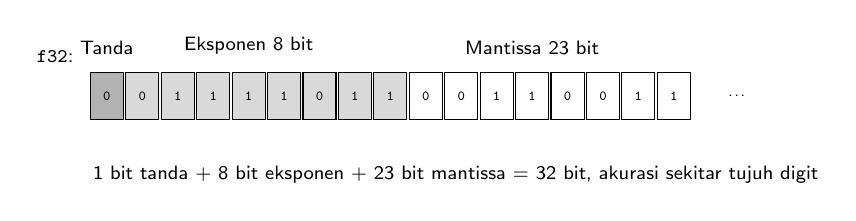
\begin{tikzpicture}[
			bit/.style={rectangle, draw=black, minimum width=0.42cm, minimum height=0.6cm, font=\ttfamily\tiny},
			grouplbl/.style={font=\scriptsize\sffamily}
		]
		\node[grouplbl, anchor=east] at (-0.3, 0.5) {\texttt{f32}:};
		\node[bit, fill=black!30] (s)  at (0,0)     {0};
		\node[bit, fill=black!15] (e1) at (0.45,0)  {0};
		\node[bit, fill=black!15] (e2) at (0.9,0)   {1};
		\node[bit, fill=black!15] (e3) at (1.35,0)  {1};
		\node[bit, fill=black!15] (e4) at (1.8,0)   {1};
		\node[bit, fill=black!15] (e5) at (2.25,0)  {1};
		\node[bit, fill=black!15] (e6) at (2.7,0)   {0};
		\node[bit, fill=black!15] (e7) at (3.15,0)  {1};
		\node[bit, fill=black!15] (e8) at (3.6,0)   {1};
		\node[bit, fill=white]    (m1) at (4.05,0)  {0};
		\node[bit, fill=white]    (m2) at (4.5,0)   {0};
		\node[bit, fill=white]    (m3) at (4.95,0)  {1};
		\node[bit, fill=white]    (m4) at (5.4,0)   {1};
		\node[bit, fill=white]    (m5) at (5.85,0)  {0};
		\node[bit, fill=white]    (m6) at (6.3,0)   {0};
		\node[bit, fill=white]    (m7) at (6.75,0)  {1};
		\node[bit, fill=white]    (m8) at (7.2,0)   {1};
		\node[font=\tiny\sffamily] at (8.0,0) {$\ldots$};

		\node[grouplbl, above=0.1cm of s]  {Tanda};
		\node[grouplbl, above=0.1cm of e4] {Eksponen 8 bit};
		\node[grouplbl, above=0.1cm of m4] {Mantissa 23 bit};

		\node[font=\scriptsize\sffamily, anchor=west] at (-0.3, -1) {1 bit tanda + 8 bit eksponen + 23 bit mantissa = 32 bit, akurasi sekitar tujuh digit};
	\end{tikzpicture}
	\caption{Layout bit IEEE-754 single precision (\texttt{f32} atau \texttt{FLOAT}).}
	\label{fig:ieee}
\end{figure}

Untuk \texttt{f64} atau \texttt{DOUBLE}, layoutnya sama tetapi ukurannya berbeda: 1 bit tanda, 11 bit eksponen, dan 52 bit mantissa, memberi akurasi sekitar enam belas digit signifikan.

\subsection{Demonstrasi di MariaDB}

\begin{lstlisting}[style=code]
CREATE TABLE demo_uang (
    harga_float   FLOAT,
    harga_double  DOUBLE,
    harga_decimal DECIMAL(12,2)
);
INSERT INTO demo_uang VALUES (10.10, 10.10, 10.10);
SELECT harga_float * 100,
       harga_double * 100,
       harga_decimal * 100
FROM demo_uang;
\end{lstlisting}

Output yang mungkin muncul:

\begin{lstlisting}[style=out]
+-------------------+--------------------+---------------------+
| harga_float * 100 | harga_double * 100 | harga_decimal * 100 |
+-------------------+--------------------+---------------------+
|        1009.99994 | 1009.9999999999999 |             1010.00 |
+-------------------+--------------------+---------------------+
\end{lstlisting}

\texttt{FLOAT} menghasilkan \texttt{1009.99994}, \texttt{DOUBLE} menghasilkan \texttt{1009.9999999999999}, hanya \texttt{DECIMAL} yang menghasilkan \texttt{1010.00} dengan tepat. Pada aplikasi keuangan, selisih enam per seratus ribu per transaksi bisa menjadi miliaran rupiah per tahun. Aturan industri: uang wajib \texttt{DECIMAL}.

\subsection{Pemetaan ke Rust dan Zig}

\begin{table}[H]
	\centering
	\caption{Pemetaan tipe float Rust dan Zig ke tipe SQL.}
	\label{tab:float}
	\small
	\begin{tabular}{l l l l l}
		\toprule
		Rust / Zig    & Bita & Padanan SQL           & Akurasi          & Kegunaan               \\
		\midrule
		\texttt{f16}  & 2    & tidak ada             & sekitar 3 digit  & ---                    \\
		\texttt{f32}  & 4    & \texttt{FLOAT}        & sekitar 7 digit  & Grafika, ML ringan     \\
		\texttt{f64}  & 8    & \texttt{DOUBLE}       & sekitar 16 digit & Ilmu fisika, kalkulasi \\
		\texttt{f128} & 16   & tidak ada             & sekitar 34 digit & ---                    \\
		---           & ---  & \texttt{DECIMAL(p,s)} & persis           & Uang, harga, rasio     \\
		\bottomrule
	\end{tabular}
\end{table}

\section{Boolean: Tipe yang Menyamar}

Baik Rust maupun Zig memiliki \texttt{bool} sebagai tipe satu byte. Di MariaDB, \texttt{BOOLEAN} hanyalah alias untuk \texttt{TINYINT(1)}.

\begin{figure}[H]
	\centering
	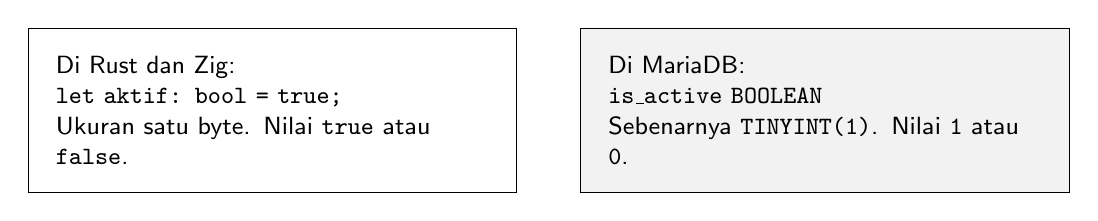
\begin{tikzpicture}[
			box/.style={rectangle, draw=black, text width=5.5cm, align=left, font=\sffamily\small, inner sep=10pt}
		]
		\node[box, fill=white] (a) {
			Di Rust dan Zig: \\
			\texttt{let aktif: bool = true;} \\
			Ukuran satu byte. Nilai \texttt{true} atau \texttt{false}.
		};
		\node[box, fill=black!5, right=0.8cm of a] (b) {
			Di MariaDB: \\
			\texttt{is\_active BOOLEAN} \\
			Sebenarnya \texttt{TINYINT(1)}. Nilai \texttt{1} atau \texttt{0}.
		};
	\end{tikzpicture}
	\caption{Perbedaan representasi boolean di Rust, Zig, dan MariaDB.}
	\label{fig:bool}
\end{figure}

Jebakan yang perlu diwaspadai: MariaDB memperlakukan nilai apa pun yang bukan nol sebagai \texttt{TRUE}.

\begin{lstlisting}[style=code]
INSERT INTO users (is_active) VALUES (5);
SELECT is_active FROM users;
\end{lstlisting}

Outputnya adalah \texttt{1}. MariaDB mengubah \texttt{5} menjadi \texttt{1} karena \texttt{BOOLEAN} hanya peduli nol atau bukan nol. Ini berbeda dengan Rust yang akan menolak \texttt{let aktif: bool = 5;} saat kompilasi.

\section{String: Mengapa \texttt{CHAR} dan \texttt{VARCHAR} Berbeda}

\subsection{Analogi Lemari Sepatu dan Rak Sepatu}

Bayangkan kamu menyimpan sepatu. Ada dua cara:

\begin{itemize}
	\item Lemari sepatu (\texttt{CHAR}): setiap kotak berukuran sama, misalnya 30 kali 30 sentimeter. Sepatu kecil tetap memakan kotak penuh. Rapi, mudah dicari, tetapi boros.
	\item Rak sepatu (\texttt{VARCHAR}): setiap sepatu menempati ruang sesuai ukurannya. Hemat, tetapi butuh label tambahan untuk menandai panjang sepatu.
\end{itemize}

Gambar~\ref{fig:char-varchar} mengilustrasikan penyimpanan kata "du" pada kedua tipe.

\begin{figure}[H]
	\centering
	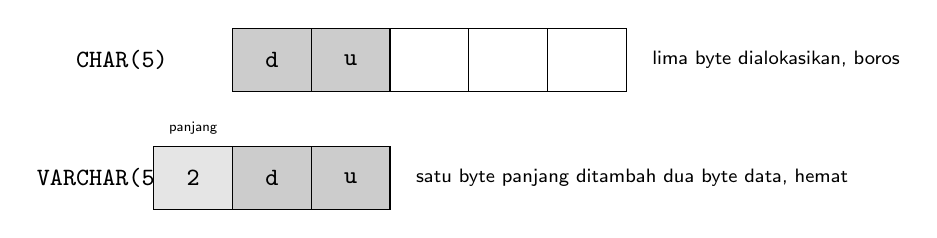
\begin{tikzpicture}[
			cell/.style={rectangle, draw=black, minimum width=1cm, minimum height=0.8cm, font=\ttfamily\small},
			label/.style={font=\sffamily\small}
		]
		\node[label, anchor=east] at (-1.2, 2) {\texttt{CHAR(5)}};
		\node[cell, fill=black!20] (c1) at (0,2) {d};
		\node[cell, fill=black!20] (c2) at (1,2) {u};
		\node[cell, fill=white]    (c3) at (2,2) { };
		\node[cell, fill=white]    (c4) at (3,2) { };
		\node[cell, fill=white]    (c5) at (4,2) { };
		\node[font=\scriptsize\sffamily, right=0.2cm of c5] {lima byte dialokasikan, boros};

		\node[label, anchor=east] at (-1.2, 0.5) {\texttt{VARCHAR(5)}};
		\node[cell, fill=black!10] (len) at (-1,0.5) {2};
		\node[font=\tiny\sffamily, above=0.02cm of len] {panjang};
		\node[cell, fill=black!20] (v1) at (0,0.5) {d};
		\node[cell, fill=black!20] (v2) at (1,0.5) {u};
		\node[font=\scriptsize\sffamily, right=0.2cm of v2] {satu byte panjang ditambah dua byte data, hemat};
	\end{tikzpicture}
	\caption{Ilustrasi alokasi memori \texttt{CHAR(5)} dan \texttt{VARCHAR(5)}.}
	\label{fig:char-varchar}
\end{figure}

\texttt{CHAR(5)} selalu memakai lima byte, sedangkan \texttt{VARCHAR(5)} memakai satu byte panjang ditambah jumlah byte aktual. Untuk "du" yang berukuran dua byte, total \texttt{VARCHAR} adalah tiga byte.

\subsection{Aturan Emas}

\begin{itemize}
	\item \texttt{CHAR(n)}: gunakan untuk data dengan panjang pasti, seperti kode negara \texttt{'ID'}, kode pos \texttt{'29461'}, atau hash hex dengan panjang tetap.
	\item \texttt{VARCHAR(n)}: gunakan untuk data dengan panjang bervariasi, seperti nama, email, dan alamat.
\end{itemize}

\subsection{Pemetaan ke Rust dan Zig}

\begin{table}[H]
	\centering
	\caption{Pemetaan tipe string Rust, Zig, dan SQL.}
	\label{tab:str}
	\small
	\begin{tabular}{l l l l}
		\toprule
		Rust                                   & Zig                                & SQL                   & Kapan Dipakai      \\
		\midrule
		\texttt{String}, \texttt{\&str} pendek & \texttt{[]u8}, \texttt{[]const u8} & \texttt{VARCHAR(255)} & Nama, email, judul \\
		\texttt{String} panjang                & \texttt{[]u8} panjang              & \texttt{TEXT}         & Deskripsi, artikel \\
		\texttt{char}                          & \texttt{u21}                       & \texttt{CHAR(1)}      & Satu codepoint     \\
		\texttt{[char; N]}                     & \texttt{[N]u8} teks                & \texttt{CHAR(N)}      & Kode tetap         \\
		\texttt{\&[u8]}                        & \texttt{[]u8} biner                & \texttt{VARBINARY(n)} & Byte mentah        \\
		\bottomrule
	\end{tabular}
\end{table}

\section{Data Biner: Untuk Hash, UUID, dan Gambar}

\subsection{Kapan Butuh Biner, Bukan Teks}

Terkadang data bukan teks, bukan angka, melainkan byte mentah. Contohnya hash password SHA-256 sepanjang tiga puluh dua byte, UUID biner sepanjang enam belas byte, gambar mini, atau kunci enkripsi.

Menyimpan hash sebagai teks hex enam puluh empat karakter, yaitu \texttt{CHAR(64)}, memakan enam puluh empat byte. Menyimpannya sebagai \texttt{BINARY(32)} hanya memakan tiga puluh dua byte. Setengahnya.

\begin{figure}[H]
	\centering
	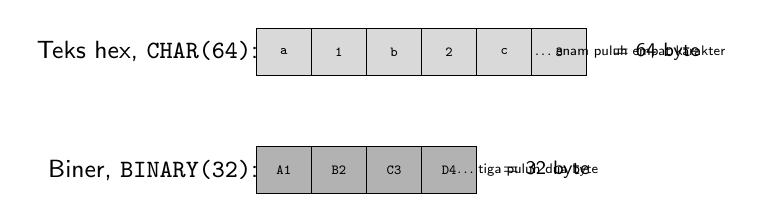
\begin{tikzpicture}[
			cell/.style={rectangle, draw=black, minimum width=0.7cm, minimum height=0.6cm, font=\ttfamily\tiny},
			label/.style={font=\sffamily\small}
		]
		\node[label, anchor=east] at (-0.2, 1) {Teks hex, \texttt{CHAR(64)}:};
		\node[cell, fill=black!15] (a1) at (0,1)   {a};
		\node[cell, fill=black!15] (a2) at (0.7,1) {1};
		\node[cell, fill=black!15] (a3) at (1.4,1) {b};
		\node[cell, fill=black!15] (a4) at (2.1,1) {2};
		\node[cell, fill=black!15] (a5) at (2.8,1) {c};
		\node[cell, fill=black!15] (a6) at (3.5,1) {3};
		\node[font=\tiny\sffamily] at (4.4,1) {$\ldots$ enam puluh empat karakter};
		\node[font=\scriptsize\sffamily, right=0.2cm of a6] {= 64 byte};

		\node[label, anchor=east] at (-0.2, -0.5) {Biner, \texttt{BINARY(32)}:};
		\node[cell, fill=black!30] (b1) at (0,-0.5)   {A1};
		\node[cell, fill=black!30] (b2) at (0.7,-0.5) {B2};
		\node[cell, fill=black!30] (b3) at (1.4,-0.5) {C3};
		\node[cell, fill=black!30] (b4) at (2.1,-0.5) {D4};
		\node[font=\tiny\sffamily] at (3.1,-0.5) {$\ldots$ tiga puluh dua byte};
		\node[font=\scriptsize\sffamily, right=0.2cm of b4] {= 32 byte};
	\end{tikzpicture}
	\caption{Perbandingan ukuran hash SHA-256 dalam teks hex dan biner.}
	\label{fig:binary}
\end{figure}

\subsection{Pemetaan ke Rust dan Zig}

\begin{table}[H]
	\centering
	\caption{Pemetaan tipe biner.}
	\label{tab:binary}
	\small
	\begin{tabular}{l l l l}
		\toprule
		Rust                      & Zig             & SQL                   & Ukuran               \\
		\midrule
		\texttt{[u8; N]}          & \texttt{[N]u8}  & \texttt{BINARY(N)}    & N byte tetap         \\
		\texttt{Vec<u8>}          & \texttt{[]u8}   & \texttt{VARBINARY(n)} & variabel, maksimum n \\
		\texttt{Vec<u8>} besar    & \texttt{[]u8}   & \texttt{BLOB}         & hingga 65.535 byte   \\
		\texttt{[u8; 16]} UUID    & \texttt{[16]u8} & \texttt{BINARY(16)}   & UUID                 \\
		\texttt{[u8; 32]} SHA-256 & \texttt{[32]u8} & \texttt{BINARY(32)}   & hash                 \\
		\bottomrule
	\end{tabular}
\end{table}

\subsection{Contoh UUID Biner}

\begin{lstlisting}[style=code]
CREATE TABLE users (
    user_id BINARY(16) PRIMARY KEY,
    nama VARCHAR(100)
);
INSERT INTO users VALUES
    (UNHEX('a1b2c3d4e5f67890a1b2c3d4e5f67890'), 'Budi');
SELECT HEX(user_id) AS user_id_hex, nama FROM users;
\end{lstlisting}

Output:

\begin{lstlisting}[style=out]
+----------------------------------+-------+
| user_id_hex                      | nama  |
+----------------------------------+-------+
| A1B2C3D4E5F67890A1B2C3D4E5F67890 | Budi  |
+----------------------------------+-------+
\end{lstlisting}

Fungsi \texttt{UNHEX()} mengubah teks hex menjadi byte mentah saat \texttt{INSERT}. Fungsi \texttt{HEX()} mengubah byte mentah kembali menjadi teks hex saat \texttt{SELECT}. Ini setara dengan \texttt{hex::encode()} dan \texttt{hex::decode()} di Rust.

\section{Tanggal dan Waktu}

\subsection{Mengapa Tanggal Tidak Boleh Disimpan sebagai Teks}

Pertanyaan ini muncul karena teks tampak lebih mudah dibaca. Tetapi menyimpan \texttt{'2026-11-02'} sebagai \texttt{VARCHAR(10)} membawa tiga konsekuensi. Pertama, operasi seperti "berapa hari lagi sampai tanggal itu" harus melalui parsing ulang setiap baris. Kedua, mengurutkan tanggal berdasarkan teks hanya bekerja untuk format ISO, dan gagal untuk format \texttt{'02/11/2026'}. Ketiga, indeks menjadi lebih besar, sepuluh byte versus tiga byte untuk \texttt{DATE}.

\begin{figure}[H]
	\centering
	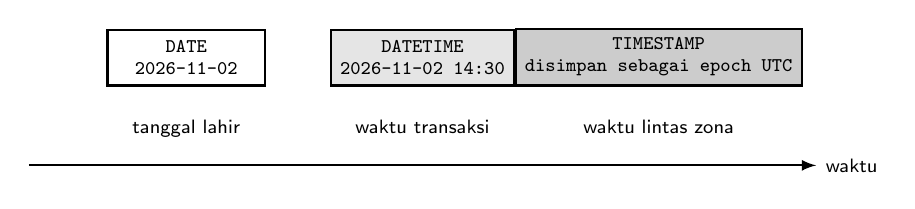
\begin{tikzpicture}[
			tl/.style={rectangle, draw=black, thick, minimum width=2cm, minimum height=0.7cm, font=\ttfamily\scriptsize, align=center}
		]
		\draw[thick, -latex] (-5,0) -- (5,0);
		\node[font=\scriptsize\sffamily, right] at (5,0) {waktu};

		\node[tl, fill=white, above=0.5cm]    (date) at (-3,0.5) {\texttt{DATE} \\ 2026-11-02};
		\node[tl, fill=black!10, above=0.5cm] (dt)   at (0,0.5)  {\texttt{DATETIME} \\ 2026-11-02 14:30};
		\node[tl, fill=black!20, above=0.5cm] (ts)   at (3,0.5)  {\texttt{TIMESTAMP} \\ disimpan sebagai epoch UTC};

		\node[font=\scriptsize\sffamily, below=0.3cm of date] {tanggal lahir};
		\node[font=\scriptsize\sffamily, below=0.3cm of dt]   {waktu transaksi};
		\node[font=\scriptsize\sffamily, below=0.3cm of ts]   {waktu lintas zona};
	\end{tikzpicture}
	\caption{Pemetaan tipe waktu pada garis waktu.}
	\label{fig:time}
\end{figure}

\subsection{Pemetaan ke Rust dan Zig}

\begin{table}[H]
	\centering
	\caption{Pemetaan tipe waktu ke Rust dan Zig.}
	\label{tab:time-map}
	\small
	\begin{tabular}{l l l l}
		\toprule
		Konsep              & SQL                & Rust                           & Zig                              \\
		\midrule
		Tanggal saja        & \texttt{DATE}      & \texttt{chrono::NaiveDate}     & \texttt{std.time.epoch}          \\
		Jam saja            & \texttt{TIME}      & \texttt{chrono::NaiveTime}     & ---                              \\
		Tanggal dan jam     & \texttt{DATETIME}  & \texttt{chrono::NaiveDateTime} & ---                              \\
		Tanggal dan jam UTC & \texttt{TIMESTAMP} & \texttt{chrono::DateTime<Utc>} & \texttt{std.time.milliTimestamp} \\
		Epoch saja          & \texttt{BIGINT}    & \texttt{i64}                   & \texttt{i64}                     \\
		\bottomrule
	\end{tabular}
\end{table}

\section{Tipe Data Khusus Modern}

\subsection{JSON}

MariaDB 10.2 ke atas mendukung tipe \texttt{JSON} yang memvalidasi struktur dan memungkinkan query dengan \texttt{JSON\_EXTRACT}. Di Rust padanannya \texttt{serde\_json::Value}, di Zig \texttt{std.json.Value}.

\begin{lstlisting}[style=code]
CREATE TABLE konfigurasi (
    user_id BIGINT UNSIGNED PRIMARY KEY,
    preferensi JSON
);
INSERT INTO konfigurasi VALUES
    (1, '{"tema":"gelap","bahasa":"id"}');
SELECT JSON_EXTRACT(preferensi, '$.tema') FROM konfigurasi;
\end{lstlisting}

Meskipun JSON memudahkan, praktik terbaiknya tetap menormalkan data ke kolom terpisah kecuali strukturnya benar-benar dinamis. JSON tidak bisa diindeks secara langsung kecuali melalui generated column, sehingga query pada JSON lebih lambat daripada query pada kolom biasa.

\subsection{UUID dan Alternatifnya}

\texttt{UUID} adalah seratus dua puluh delapan bit angka yang secara praktis unik. Di MariaDB, UUID tidak memiliki tipe native, sehingga disimpan sebagai \texttt{CHAR(36)} atau \texttt{BINARY(16)}.

Alternatif yang lebih baik untuk primary key adalah \texttt{UUID\_SHORT()}, fungsi MariaDB yang mengembalikan enam puluh empat bit monotonik. Keunggulan monotonik: nilai baru selalu bertambah, sehingga penambahan data baru selalu di ujung indeks dan menghindari fragmentasi.

\begin{figure}[H]
	\centering
	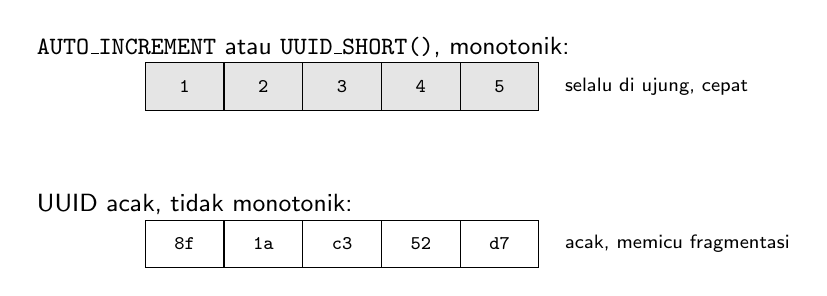
\begin{tikzpicture}[
			item/.style={rectangle, draw=black, minimum width=1cm, minimum height=0.6cm, font=\ttfamily\scriptsize}
		]
		\node[font=\sffamily\small, anchor=west] at (-5, 2) {\texttt{AUTO\_INCREMENT} atau \texttt{UUID\_SHORT()}, monotonik:};
		\node[item, fill=black!10] (a1) at (-3,1.5) {1};
		\node[item, fill=black!10] (a2) at (-2,1.5) {2};
		\node[item, fill=black!10] (a3) at (-1,1.5) {3};
		\node[item, fill=black!10] (a4) at (0,1.5)  {4};
		\node[item, fill=black!10] (a5) at (1,1.5)  {5};
		\node[font=\scriptsize\sffamily, right=0.2cm of a5] {selalu di ujung, cepat};

		\node[font=\sffamily\small, anchor=west] at (-5, 0) {UUID acak, tidak monotonik:};
		\node[item, fill=white] (b1) at (-3,-0.5) {8f};
		\node[item, fill=white] (b2) at (-2,-0.5) {1a};
		\node[item, fill=white] (b3) at (-1,-0.5) {c3};
		\node[item, fill=white] (b4) at (0,-0.5)  {52};
		\node[item, fill=white] (b5) at (1,-0.5)  {d7};
		\node[font=\scriptsize\sffamily, right=0.2cm of b5] {acak, memicu fragmentasi};
	\end{tikzpicture}
	\caption{Perbandingan pola penambahan ID monotonik dan acak.}
	\label{fig:uuid}
\end{figure}

\section{Tabel Referensi Silang Lengkap}

\begin{table}[H]
	\centering
	\caption{Tabel referensi silang lengkap Rust, Zig, dan SQL.}
	\label{tab:master}
	\footnotesize
	\begin{tabularx}{\textwidth}{l l l X}
		\toprule
		Rust                            & Zig                     & SQL                        & Keterangan                \\
		\midrule
		\texttt{u8}                     & \texttt{u8}             & \texttt{TINYINT UNSIGNED}  & 1 byte, 0--255            \\
		\texttt{i8}                     & \texttt{i8}             & \texttt{TINYINT}           & 1 byte, $-128$--$127$     \\
		\texttt{u16}                    & \texttt{u16}            & \texttt{SMALLINT UNSIGNED} & 2 byte                    \\
		\texttt{i16}                    & \texttt{i16}            & \texttt{SMALLINT}          & 2 byte                    \\
		\texttt{u32}                    & \texttt{u32}            & \texttt{INT UNSIGNED}      & 4 byte                    \\
		\texttt{i32}                    & \texttt{i32}            & \texttt{INT}               & 4 byte                    \\
		\texttt{u64}                    & \texttt{u64}            & \texttt{BIGINT UNSIGNED}   & 8 byte                    \\
		\texttt{i64}                    & \texttt{i64}            & \texttt{BIGINT}            & 8 byte                    \\
		\texttt{u128}                   & \texttt{u128}           & \texttt{DECIMAL(39,0)}     & tidak native              \\
		\texttt{f32}                    & \texttt{f32}            & \texttt{FLOAT}             & IEEE-754 32 bit           \\
		\texttt{f64}                    & \texttt{f64}            & \texttt{DOUBLE}            & IEEE-754 64 bit           \\
		\texttt{bool}                   & \texttt{bool}           & \texttt{BOOLEAN}           & alias \texttt{TINYINT(1)} \\
		\texttt{char}                   & \texttt{u21}            & \texttt{CHAR(1)}           & satu codepoint            \\
		\texttt{String}, \texttt{\&str} & \texttt{[]u8}           & \texttt{VARCHAR(n)}        & teks variabel             \\
		\texttt{String} panjang         & \texttt{[]u8} panjang   & \texttt{TEXT}              & teks panjang              \\
		\texttt{[u8; N]}                & \texttt{[N]u8}          & \texttt{BINARY(N)}         & byte tetap                \\
		\texttt{Vec<u8>}                & \texttt{[]u8}           & \texttt{VARBINARY(n)}      & byte variabel             \\
		\texttt{Option<T>}              & \texttt{?T}             & \texttt{NULL}              & kolom nullable            \\
		\texttt{chrono::NaiveDate}      & \texttt{std.time.epoch} & \texttt{DATE}              & tanggal                   \\
		\texttt{chrono::NaiveDateTime}  & ---                     & \texttt{DATETIME}          & tanggal dan jam           \\
		\texttt{serde\_json::Value}     & \texttt{std.json.Value} & \texttt{JSON}              & data semi-terstruktur     \\
		\texttt{uuid::Uuid}             & \texttt{[16]u8}         & \texttt{BINARY(16)}        & UUID biner                \\
		\bottomrule
	\end{tabularx}
\end{table}

\section{Pohon Keputusan}

\begin{figure}[H]
	\centering
	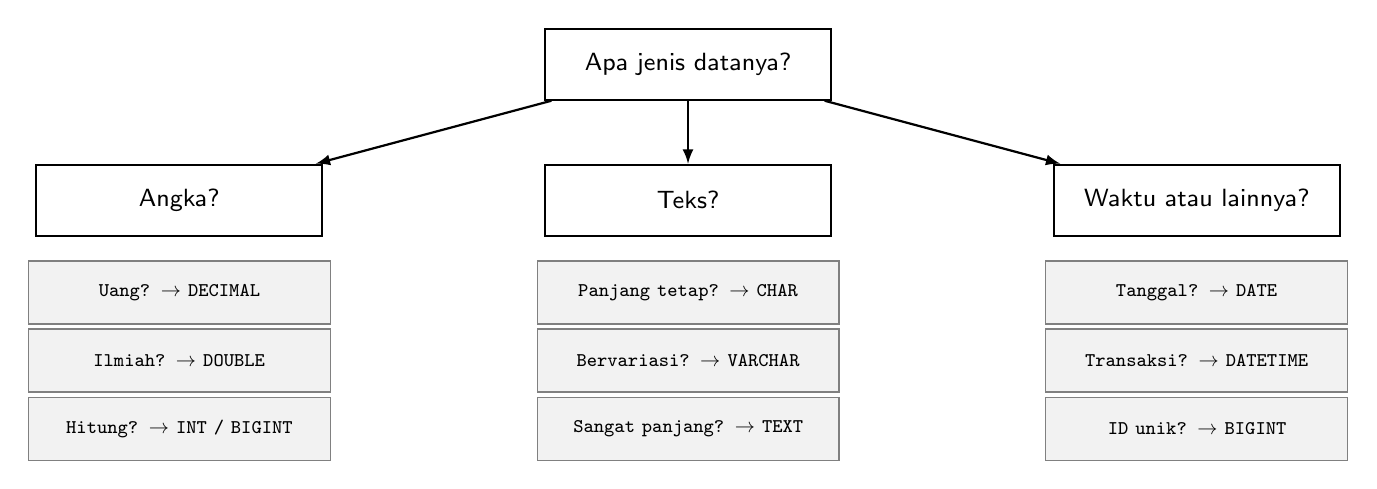
\begin{tikzpicture}[
			node distance=0.4cm and 0.6cm,
			q/.style={rectangle, draw=black, thick, fill=white, text width=3.4cm, align=center, minimum height=0.9cm, font=\sffamily\small},
			a/.style={rectangle, draw=black!50, fill=black!5, text width=3.6cm, align=center, minimum height=0.8cm, font=\ttfamily\scriptsize},
			line/.style={draw, thick, -latex}
		]
		\node[q] (start) {Apa jenis datanya?};
		\node[q, below left=0.8cm and 2.8cm of start] (num) {Angka?};
		\node[q, below=0.8cm of start] (str) {Teks?};
		\node[q, below right=0.8cm and 2.8cm of start] (other) {Waktu atau lainnya?};

		\draw[line] (start) -- (num);
		\draw[line] (start) -- (str);
		\draw[line] (start) -- (other);

		\node[a, below=0.3cm of num] (n1) {Uang? $\rightarrow$ \texttt{DECIMAL}};
		\node[a, below=0.05cm of n1] (n2) {Ilmiah? $\rightarrow$ \texttt{DOUBLE}};
		\node[a, below=0.05cm of n2] (n3) {Hitung? $\rightarrow$ \texttt{INT / BIGINT}};

		\node[a, below=0.3cm of str] (s1) {Panjang tetap? $\rightarrow$ \texttt{CHAR}};
		\node[a, below=0.05cm of s1] (s2) {Bervariasi? $\rightarrow$ \texttt{VARCHAR}};
		\node[a, below=0.05cm of s2] (s3) {Sangat panjang? $\rightarrow$ \texttt{TEXT}};

		\node[a, below=0.3cm of other] (o1) {Tanggal? $\rightarrow$ \texttt{DATE}};
		\node[a, below=0.05cm of o1] (o2) {Transaksi? $\rightarrow$ \texttt{DATETIME}};
		\node[a, below=0.05cm of o2] (o3) {ID unik? $\rightarrow$ \texttt{BIGINT}};
	\end{tikzpicture}
	\caption{Pohon keputusan pemilihan tipe data.}
	\label{fig:decision}
\end{figure}

\section{Kesalahan Umum}

\begin{table}[H]
	\centering
	\caption{Kesalahan umum dalam memilih tipe data.}
	\label{tab:mistakes}
	\footnotesize
	\begin{tabularx}{\textwidth}{l X X}
		\toprule
		Kesalahan                          & Akibat                            & Perbaikan                                    \\
		\midrule
		\texttt{FLOAT} untuk uang          & selisih sen menumpuk menjadi juta & gunakan \texttt{DECIMAL}                     \\
		\texttt{CHAR(255)} untuk nama      & boros 253 byte per baris          & gunakan \texttt{VARCHAR(50)}                 \\
		\texttt{BIGINT} untuk umur         & indeks membengkak dua kali        & gunakan \texttt{TINYINT UNSIGNED}            \\
		tanggal sebagai \texttt{VARCHAR}   & sortir dan aritmatika lambat      & gunakan \texttt{DATE} atau \texttt{DATETIME} \\
		\texttt{CHAR(36)} untuk UUID       & boros 20 byte per baris           & gunakan \texttt{BINARY(16)}                  \\
		hash password di \texttt{CHAR(64)} & boros 32 byte per baris           & gunakan \texttt{BINARY(32)}                  \\
		\texttt{TEXT} untuk kolom filter   & indeks tidak bisa dipakai penuh   & gunakan \texttt{VARCHAR(255)}                \\
		\texttt{AUTO\_INCREMENT} terbuka   & ID mudah ditebak, rawan scraping  & gunakan \texttt{UUID\_SHORT()}               \\
		\bottomrule
	\end{tabularx}
\end{table}

\section{Studi Kasus: Merancang Tabel \texttt{users}}

Mari rangkai seluruh konsep dalam satu tabel produksi. Setiap kolom dipilih dengan alasan eksplisit.

\begin{lstlisting}[style=code]
CREATE TABLE users (
    user_id       BIGINT UNSIGNED DEFAULT (UUID_SHORT()) PRIMARY KEY,
    username      VARCHAR(50)     NOT NULL UNIQUE,
    email         VARCHAR(255)    NOT NULL UNIQUE,
    password_hash BINARY(32)      NOT NULL,
    tanggal_lahir DATE,
    is_active     BOOLEAN         NOT NULL DEFAULT TRUE,
    saldo         DECIMAL(15,2)   NOT NULL DEFAULT 0.00,
    metadata      JSON,
    created_at    DATETIME        DEFAULT CURRENT_TIMESTAMP,
    updated_at    DATETIME        DEFAULT CURRENT_TIMESTAMP
                                  ON UPDATE CURRENT_TIMESTAMP
);
\end{lstlisting}

Bedah pilihan per kolom:

\begin{itemize}
	\item \texttt{user\_id BIGINT UNSIGNED}: setara \texttt{u64}. \texttt{UUID\_SHORT()} monotonik, anti-fragmentasi, lebih cepat dari \texttt{CHAR(36)}.
	\item \texttt{username VARCHAR(50)}: panjang bervariasi, wajib diisi, harus unik.
	\item \texttt{email VARCHAR(255)}: batas 255 sesuai RFC 5321.
	\item \texttt{password\_hash BINARY(32)}: hash SHA-256 biner, setara \texttt{[u8; 32]}. Hemat 32 byte dibanding \texttt{CHAR(64)}.
	\item \texttt{tanggal\_lahir DATE}: hanya tanggal, tanpa jam.
	\item \texttt{is\_active BOOLEAN}: alias \texttt{TINYINT(1)}.
	\item \texttt{saldo DECIMAL(15,2)}: uang, wajib exact numeric.
	\item \texttt{metadata JSON}: data semi-terstruktur opsional.
	\item \texttt{created\_at DATETIME}: otomatis saat \texttt{INSERT}.
	\item \texttt{updated\_at DATETIME ON UPDATE}: otomatis berubah saat \texttt{UPDATE}.
\end{itemize}

Coba \texttt{INSERT} tanpa menyebut kolom yang punya \texttt{DEFAULT}:

\begin{lstlisting}[style=code]
INSERT INTO users (username, email, password_hash)
VALUES ('budi', 'budi@email.com', UNHEX(REPEAT('ab', 32)));
\end{lstlisting}

Semua kolom lain akan terisi otomatis: \texttt{user\_id}, \texttt{is\_active}, \texttt{saldo}, \texttt{created\_at}, dan \texttt{updated\_at}. Inilah kekuatan \texttt{DEFAULT} yang dikombinasikan dengan ekspresi.

\section{Lembar Rujukan Cepat}

\begin{table}[H]
	\centering
	\caption{Lembar rujukan cepat memilih tipe data.}
	\label{tab:cheat}
	\footnotesize
	\begin{tabularx}{\textwidth}{l X}
		\toprule
		Kebutuhan                   & Tipe yang Tepat                                        \\
		\midrule
		status aktif atau nonaktif  & \texttt{BOOLEAN}, alias \texttt{TINYINT(1)}            \\
		umur, jumlah anak           & \texttt{TINYINT UNSIGNED}                              \\
		jumlah barang               & \texttt{INT UNSIGNED}                                  \\
		ID pengguna                 & \texttt{BIGINT UNSIGNED} dengan \texttt{UUID\_SHORT()} \\
		harga, saldo, pajak         & \texttt{DECIMAL(15,2)}                                 \\
		koordinat GPS               & \texttt{DECIMAL(9,6)}                                  \\
		berat badan                 & \texttt{DECIMAL(5,2)}                                  \\
		nama orang                  & \texttt{VARCHAR(100)}                                  \\
		email                       & \texttt{VARCHAR(255)}                                  \\
		alamat                      & \texttt{VARCHAR(500)}                                  \\
		deskripsi produk            & \texttt{TEXT}                                          \\
		kode negara                 & \texttt{CHAR(2)}                                       \\
		kode pos Indonesia          & \texttt{CHAR(5)}                                       \\
		tanggal lahir               & \texttt{DATE}                                          \\
		waktu transaksi             & \texttt{DATETIME}                                      \\
		waktu lintas zona waktu     & \texttt{TIMESTAMP}                                     \\
		hash password               & \texttt{BINARY(32)}                                    \\
		UUID                        & \texttt{BINARY(16)}                                    \\
		konfigurasi aplikasi        & \texttt{JSON}                                          \\
		gambar kecil di bawah 64 KB & \texttt{BLOB}                                          \\
		\bottomrule
	\end{tabularx}
\end{table}

\section{Kesimpulan}

Tipe data SQL bukanlah daftar hafalan yang terpisah dari dunia pemrograman sistem. Ia adalah cermin dari tipe primitif yang sudah dikenal di Rust dan Zig. Tiga prinsip penutup:

\begin{enumerate}
	\item Integer: pilih yang terkecil yang cukup. \texttt{INT} lebih baik daripada \texttt{BIGINT} jika nilai tidak akan melewati empat miliar, karena setiap indeks sekunder menyalin ukuran tersebut.
	\item Uang: wajib \texttt{DECIMAL}. Jangan pernah menggunakan \texttt{FLOAT} atau \texttt{DOUBLE} untuk nilai moneter.
	\item Teks dan biner: \texttt{CHAR} untuk panjang tetap, \texttt{VARCHAR} untuk variabel, \texttt{BINARY(n)} untuk byte mentah. Untuk hash dan UUID, gunakan bentuk biner, bukan teks hex.
\end{enumerate}

Dengan kerangka mental ini, keputusan memilih tipe data menjadi keputusan arsitektural yang sadar, bukan sekadar "yang penting bisa jalan".

\newpage
\section*{Referensi}
\addcontentsline{toc}{section}{Referensi}

\begin{thebibliography}{99}
	\bibitem{rust} The Rust Project Developers. (2026). \textit{Data Types --- The Rust Programming Language}. \texttt{https://doc.rust-lang.org/book/ch03-02-data-types.html}.
	\bibitem{zig} Zig Software Foundation. (2026). \textit{Language Reference --- Primitive Types}. \texttt{https://ziglang.org/documentation/master/}.
	\bibitem{mariadb-types} MariaDB Foundation. (2026). \textit{Data Types}. MariaDB Knowledge Base. \texttt{https://mariadb.com/kb/en/data-types/}.
	\bibitem{mysql-types} Oracle Corporation. (2026). \textit{MySQL 8.0 Reference Manual --- Data Types}. \texttt{https://dev.mysql.com/doc/refman/8.0/en/data-types.html}.
	\bibitem{postgresql} The PostgreSQL Global Development Group. (2026). \textit{Chapter 8. Data Types}. \texttt{https://www.postgresql.org/docs/current/datatype.html}.
	\bibitem{microsoft} Microsoft. (2026). \textit{Data Types (Transact-SQL)}. Microsoft Learn. \texttt{https://learn.microsoft.com/en-us/sql/t-sql/data-types/}.
	\bibitem{ieee754} IEEE. (2019). \textit{IEEE Standard for Floating-Point Arithmetic (IEEE 754-2019)}. Institute of Electrical and Electronics Engineers.
	\bibitem{silberschatz} Silberschatz, A., Korth, H. F., \& Sudarshan, S. (2019). \textit{Database System Concepts} (7th ed.). McGraw-Hill Education.
	\bibitem{date} Date, C. J. (2003). \textit{An Introduction to Database Systems} (8th ed.). Addison-Wesley.
	\bibitem{kleppmann} Kleppmann, M. (2017). \textit{Designing Data-Intensive Applications}. O'Reilly Media.
	\bibitem{rfc4122} Leach, P., Mealling, M., \& Salz, R. (2005). \textit{A Universally Unique IDentifier (UUID) URN Namespace} (RFC 4122). IETF.
	\bibitem{rfc5321} Klensin, J. (2008). \textit{Simple Mail Transfer Protocol} (RFC 5321). IETF.
\end{thebibliography}

\end{document}
